\section{HDR ML Anomaly Challenge (Gravitational Waves)}
{{\footnotesize
\begin{description}[labelwidth=5em, labelsep=1em, leftmargin=*, align=left, itemsep=0.3em, parsep=0em]
  \item[date:] 2025-03-03
  \item[last\_updated:] 2025-03
  \item[expired:] unkown
  \item[valid:] yes
  \item[url:] \href{https://www.codabench.org/competitions/2626/}{https://www.codabench.org/competitions/2626/}
  \item[domain:] Astrophysics; Time-series
  \item[focus:] Detecting anomalous gravitational-wave signals from LIGO/Virgo datasets
  \item[keywords:]
    - anomaly detection
    - gravitational waves
    - astrophysics
    - time-series
  \item[task\_types:]
    - Anomaly detection
  \item[ai\_capability\_measured:]
    - Novel event detection in physical signals
  \item[metrics:]
    - ROC‑AUC
    - Precision/Recall
  \item[models:]
    - Deep latent CNNs
    - Autoencoders
  \item[ml\_motif:]
    - Time-series
  \item[type:] Dataset
  \item[ml\_task:] Anomaly detection
  \item[notes:] NSF HDR A3D3 sponsored; prize pool and starter kit provided on Codabench. :contentReference[oaicite:2]\{index=2\}
  \item[contact.name:] HDR A3D3 Team
  \item[contact.email:] unkown
  \item[results.name:] ChatGPT LLM
  \item[results.url:] \href{unkown}{unkown}
  \item[fair.reproducible:] Yes
  \item[fair.benchmark\_ready:] Yes
  \item[ratings.software.rating:] 0
  \item[ratings.software.reason:] Not analyzed.
  \item[ratings.specification.rating:] 8.0
  \item[ratings.specification.reason:] Novel approach treating forecasting as text generation is explained; framing is less conventional.
  \item[ratings.dataset.rating:] 9.0
  \item[ratings.dataset.reason:] Compatible with standard forecasting datasets (e.g., M4, electricity).
  \item[ratings.metrics.rating:] 8.0
  \item[ratings.metrics.reason:] RMSE and MAPE are included, but less emphasis on interpretability or time-series domain constraints.
  \item[ratings.reference\_solution.rating:] 9.0
  \item[ratings.reference\_solution.reason:] Open-source with reprogramming layers, LLM interface scripts provided.
  \item[ratings.documentation.rating:] 8.0
  \item[ratings.documentation.reason:] Model and architecture overview present, though usability guide is slightly lighter than others.
  \item[id:] hdr\_ml\_anomaly\_challenge\_gravitational\_waves
  \item[Citations:] \cite{campolongo2025buildingmachinelearningchallenges}
  \item[Ratings:]
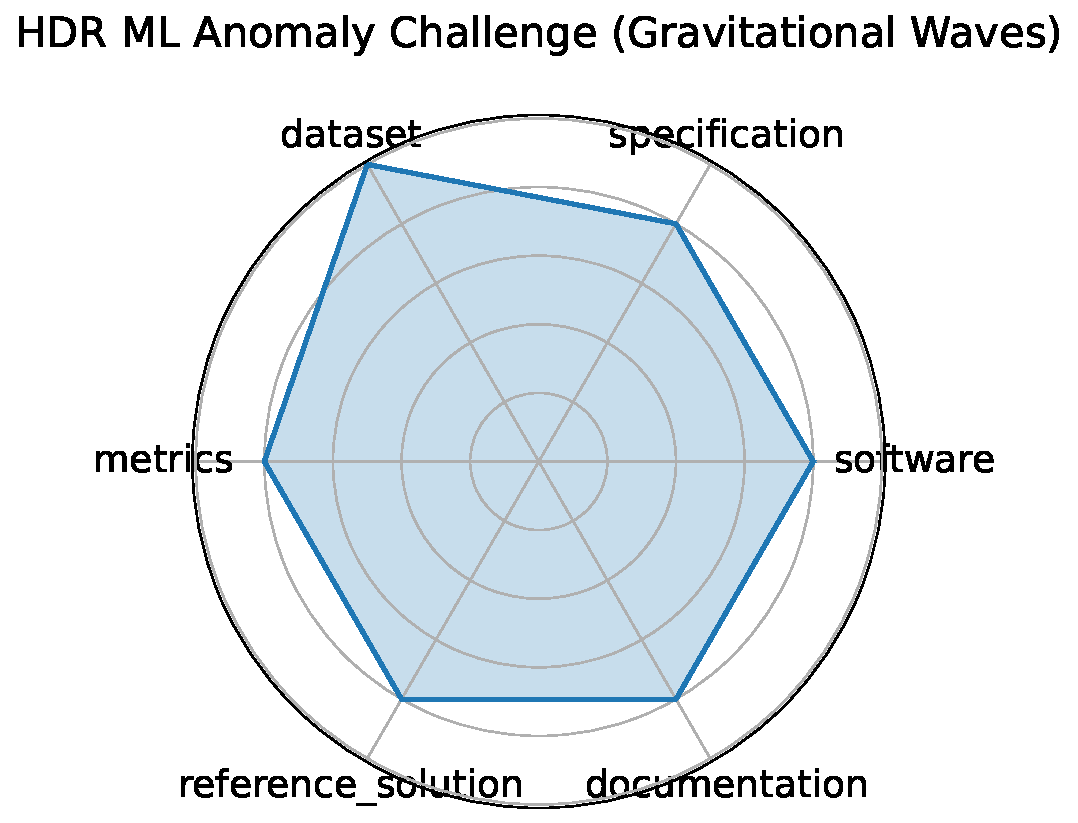
\includegraphics[width=0.2\textwidth]{hdr_ml_anomaly_challenge_gravitational_waves_radar.pdf}
\end{description}
}}
\clearpage